\label{chap:introduction}
\ac{WHO} figures claim that as as of 2012, there are 285 million people suffering from visual imparements~\cite{whoblindness}, 30 million of whom are blind. The \ac{WHO} also state that 90\% of the visually impaired live in developing countries. Combined with statistics from the guide dogs for the blind association, who claim that the life-time cost of training and keeping a guide dog is around \pounds50,000, a sad picture is painted the majority who are unable to afford such visual aids.

\section{Aims, Goals and Contributions}
This project aims to develop a method of conveying visual information without the user of the system requiring a functional visual system. The study investigates both navigational and semantic modes of operation, and the different techniques associated with each implementation.

The system should be cheaper than current traditional solutions (such as guide-dogs), and be more effective than the more ``high-tech'' solutions detailed in section \ref{sec:existing}.

The report details a functional system, which is able to be used to effectively navigate around a room and avoid obstacles without the use of eyes. Additionally, the system details the pros and cons of various methods of shape classification and parameterisation, with the view to sonification. 

\section{Intended Audience}
The main intended audience for this project is the visually impaired. It is anticipated that the ``tech savvy'' visually impaired would be interested in trialling the prototypes, both for day-to-day use, and to assist in further development.

\begin{figure}[H]
    \centering
    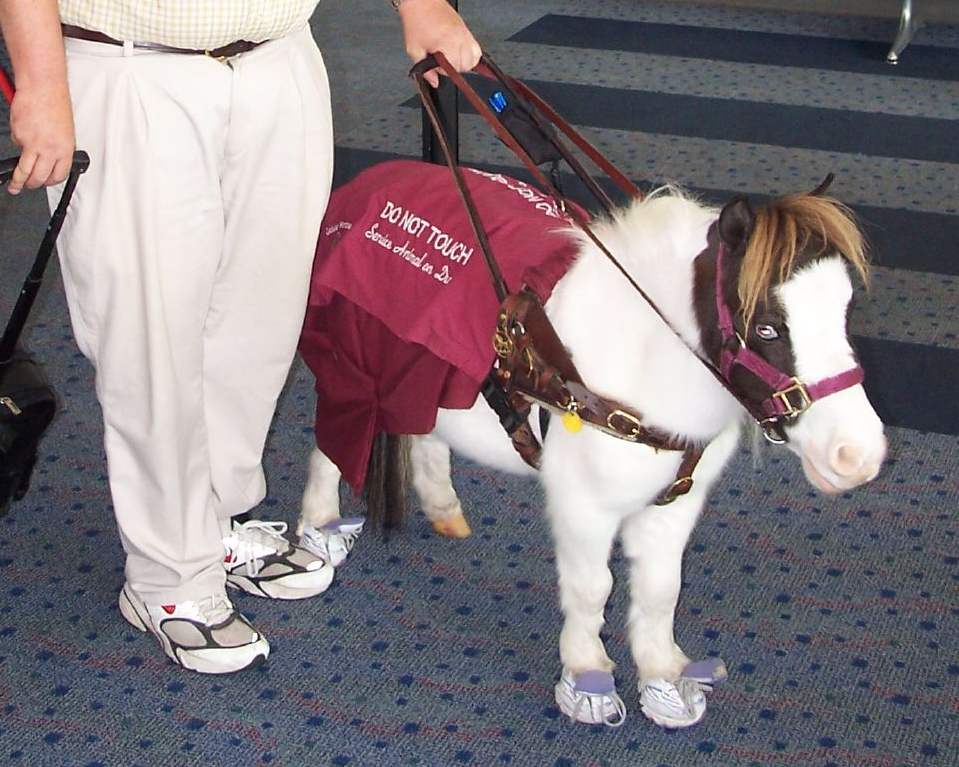
\includegraphics[width=0.5\textwidth]{Introduction/guidehorse.png}
    \caption{A guidehorse (source: Wikimedia Commons)}
\end{figure}

The system is not intended to replace all other forms of visual assistance --- rather, it intends to assist those who are unable to afford luxuries such as Guide-dogs or Guide-horses~\cite{guidehorse}. A low-cost system that is capable of assisting a user in navigating a room and detecting obstacles has the potential to be life changing --- even if only a small fraction of a normal, functional visual system can be imitated, 0.01\% is infinitely greater than 0.00\%~\cite{dawkins1996blind}.

\section{Project Scope}
The project has a fairly broad scope, and includes:
\begin{description}
    \item[Image Segmentation] This deals with the extracting the input image, and extracting an object of interest
    \item[Descriptor Extraction] This is the extraction of descriptors from the object of interest (obtained from step 1)
    \item[Descriptor Sonification] Sonification of the output from step 2.
\end{description}

Components/considerations \textbf{outside} of the scope of this project are:
\begin{description}
    \item[Camera Evaluation] Detailed evaluation of specific models of depth-sensing cameras is out of the scope of this project. 
    \item[Robust Testing] It is not anticipated that the system described in this report go into immediate production -- in-depth safety testing is out-of-scope. 
    \item[In-depth UX/UI development] The UI should be functional, but UI usability is not the primary focus of the project. 
\end{description}

\section{Approach}
I took a parallel approach while researching my solution to the problem. Rather than carry out work step-by-step, where problems and delays could have had a serious impact on the project schedule, work was carried out asynchronously to help mitigate such risks. 

\section{Assumptions}
Several assumptions have been made during the development of the software. Firstly, it is assumed that the system will be used indoors. The Asus Xtion Pro Live camera~\cite{xtion} chosen for use in the project uses \ac{IR} laser light to measure distance. In direct sunlight, the \ac{IR} radiation emitted by the sun over-powers the \ac{IR} light emitted by the Xtion, resulting in in-accurate readings. This is a limitation of a majority of \ac{RGB-D} cameras using structured light or time-of-flight, although future work could involve the use of a stereoscopic camera setup as a solution to the problem.

Secondly, as the systems described in this report convey information in the form of audio, it is assumed that the user of the system has a functional auditory system. Although there is a percentage of the population that are both deaf AND blind, a majority of the blind have at least some auditory functionality.

Additionally, it is assumed that the potential user of the system would be willing to carry a portable computer (i.e. laptop) and Xtion Camera during it's operation.
